\chapter{Desenvolvimento}\label{cap:CnptDsng}

\section{Obstáculos}\label{sec:arqgrl}
O primeiro passado adotado foi a análise dos pontos, verificando se entre os dois existia algum obstáculo. Essa informação pode ser extraída dos mapas que foram fornecidos em anexo, como mostra a figura \ref{fig:obs_cam}.
\begin{figure}[h]
	\centering
	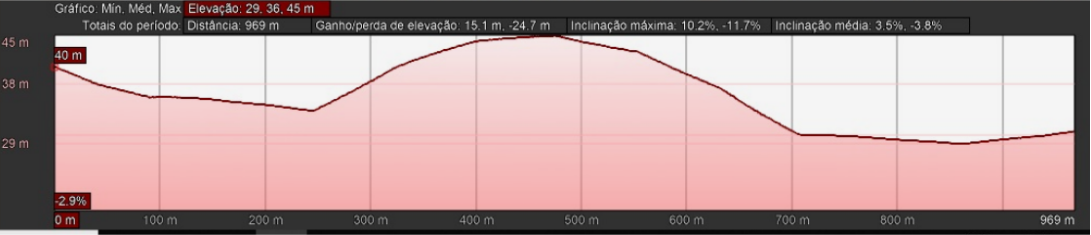
\includegraphics[width=1\textwidth]{obs_cam.png}
	\caption{Gráfico de obstáculo}
	\label{fig:obs_cam}
	\source{Própria}
\end{figure} 

Por meio da análise do gráfico, fica evidenciado que entre os dois pontos existe um grande obstáculo arredondado, assim sendo necessário calcular o seu raio de curvatura e a partir disso ver o quanto ele irá interferir na transmissão.
É feita uma aproximação do topo do obstáculo, utilizando uma curvatura parabólica como mostrado na figura \ref{fig:obs_raio}.

\begin{figure}[h]
	\centering
	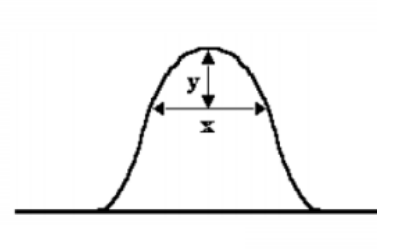
\includegraphics[width=1\textwidth]{obs_raio.png}
	\caption{Gráfico de obstáculo}
	\label{fig:obs_raio}
	\caption{Curvatura parabólica utilizada para aproximação}
	\source{Própria}
\end{figure} 

O raio $r$ da parábola será calculado o $\alpha$ que possibilita encontrar quantos decibéis de interferência o obstáculo irá causar. O cálculo do raio $r$ é feito utilizando a seguinte formula:
\begin{equation}
r = {x^2/8*y}*10^{-3}
\end{equation}












